\documentclass[border=4pt]{standalone}

\usepackage{amsmath}
\usepackage{tikz}
\usepackage{mathdots}
\usepackage{yhmath}
\usepackage{cancel}
\usepackage{color}
\usepackage{siunitx}
\usepackage{array}
\usepackage{multirow}
\usepackage{amssymb}
\usepackage{gensymb}
\usepackage{tabularx}
\usepackage{booktabs}
\usetikzlibrary{fadings}
\usetikzlibrary{patterns}


\begin{document}
 


\tikzset{every picture/.style={line width=0.75pt}} %set default line width to 0.75pt        

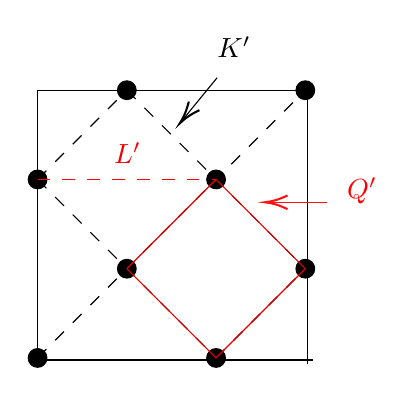
\begin{tikzpicture}[x=0.75pt,y=0.75pt,yscale=-1,xscale=1]
%uncomment if require: \path (0,348); %set diagram left start at 0, and has height of 348

%Shape: Grid [id:dp21285255618878818] 
\draw  [draw opacity=0] (180,70) -- (312.5,70) -- (312.5,202) -- (180,202) -- cycle ; \draw   (180,70) -- (180,202)(310,70) -- (310,202) ; \draw   (180,70) -- (312.5,70)(180,200) -- (312.5,200) ; \draw    ;
%Shape: Circle [id:dp9352280486568025] 
\draw  [color={rgb, 255:red, 0; green, 0; blue, 0 }  ,draw opacity=1 ][fill={rgb, 255:red, 0; green, 0; blue, 0 }  ,fill opacity=1 ] (175.5,113) .. controls (175.5,110.51) and (177.51,108.5) .. (180,108.5) .. controls (182.49,108.5) and (184.5,110.51) .. (184.5,113) .. controls (184.5,115.49) and (182.49,117.5) .. (180,117.5) .. controls (177.51,117.5) and (175.5,115.49) .. (175.5,113) -- cycle ;
%Shape: Circle [id:dp16026326261630874] 
\draw  [color={rgb, 255:red, 0; green, 0; blue, 0 }  ,draw opacity=1 ][fill={rgb, 255:red, 0; green, 0; blue, 0 }  ,fill opacity=1 ] (218.5,70) .. controls (218.5,67.51) and (220.51,65.5) .. (223,65.5) .. controls (225.49,65.5) and (227.5,67.51) .. (227.5,70) .. controls (227.5,72.49) and (225.49,74.5) .. (223,74.5) .. controls (220.51,74.5) and (218.5,72.49) .. (218.5,70) -- cycle ;
%Shape: Circle [id:dp5085921771663904] 
\draw  [color={rgb, 255:red, 0; green, 0; blue, 0 }  ,draw opacity=1 ][fill={rgb, 255:red, 0; green, 0; blue, 0 }  ,fill opacity=1 ] (218.5,156) .. controls (218.5,153.51) and (220.51,151.5) .. (223,151.5) .. controls (225.49,151.5) and (227.5,153.51) .. (227.5,156) .. controls (227.5,158.49) and (225.49,160.5) .. (223,160.5) .. controls (220.51,160.5) and (218.5,158.49) .. (218.5,156) -- cycle ;
%Shape: Circle [id:dp4967973034032702] 
\draw  [color={rgb, 255:red, 0; green, 0; blue, 0 }  ,draw opacity=1 ][fill={rgb, 255:red, 0; green, 0; blue, 0 }  ,fill opacity=1 ] (261.5,113) .. controls (261.5,110.51) and (263.51,108.5) .. (266,108.5) .. controls (268.49,108.5) and (270.5,110.51) .. (270.5,113) .. controls (270.5,115.49) and (268.49,117.5) .. (266,117.5) .. controls (263.51,117.5) and (261.5,115.49) .. (261.5,113) -- cycle ;
%Shape: Circle [id:dp11814545059064674] 
\draw  [color={rgb, 255:red, 0; green, 0; blue, 0 }  ,draw opacity=1 ][fill={rgb, 255:red, 0; green, 0; blue, 0 }  ,fill opacity=1 ] (175.5,199) .. controls (175.5,196.51) and (177.51,194.5) .. (180,194.5) .. controls (182.49,194.5) and (184.5,196.51) .. (184.5,199) .. controls (184.5,201.49) and (182.49,203.5) .. (180,203.5) .. controls (177.51,203.5) and (175.5,201.49) .. (175.5,199) -- cycle ;
%Shape: Circle [id:dp7267703003097346] 
\draw  [color={rgb, 255:red, 0; green, 0; blue, 0 }  ,draw opacity=1 ][fill={rgb, 255:red, 0; green, 0; blue, 0 }  ,fill opacity=1 ] (261.5,199) .. controls (261.5,196.51) and (263.51,194.5) .. (266,194.5) .. controls (268.49,194.5) and (270.5,196.51) .. (270.5,199) .. controls (270.5,201.49) and (268.49,203.5) .. (266,203.5) .. controls (263.51,203.5) and (261.5,201.49) .. (261.5,199) -- cycle ;
%Shape: Circle [id:dp0648619648322224] 
\draw  [color={rgb, 255:red, 0; green, 0; blue, 0 }  ,draw opacity=1 ][fill={rgb, 255:red, 0; green, 0; blue, 0 }  ,fill opacity=1 ] (304.5,156) .. controls (304.5,153.51) and (306.51,151.5) .. (309,151.5) .. controls (311.49,151.5) and (313.5,153.51) .. (313.5,156) .. controls (313.5,158.49) and (311.49,160.5) .. (309,160.5) .. controls (306.51,160.5) and (304.5,158.49) .. (304.5,156) -- cycle ;
%Shape: Circle [id:dp04555002191252555] 
\draw  [color={rgb, 255:red, 0; green, 0; blue, 0 }  ,draw opacity=1 ][fill={rgb, 255:red, 0; green, 0; blue, 0 }  ,fill opacity=1 ] (304.5,70) .. controls (304.5,67.51) and (306.51,65.5) .. (309,65.5) .. controls (311.49,65.5) and (313.5,67.51) .. (313.5,70) .. controls (313.5,72.49) and (311.49,74.5) .. (309,74.5) .. controls (306.51,74.5) and (304.5,72.49) .. (304.5,70) -- cycle ;
%Straight Lines [id:da4361917845123868] 
\draw  [dash pattern={on 4.5pt off 4.5pt}]  (223,70) -- (309,156) ;


%Straight Lines [id:da8541933437596527] 
\draw  [dash pattern={on 4.5pt off 4.5pt}]  (180,113) -- (266,199) ;


%Straight Lines [id:da4956622351456581] 
\draw  [dash pattern={on 4.5pt off 4.5pt}]  (180,199) -- (309,70) ;


%Straight Lines [id:da17935623392185351] 
\draw  [dash pattern={on 4.5pt off 4.5pt}]  (180,113) -- (223,70) ;


%Straight Lines [id:da8939529391952115] 
\draw  [dash pattern={on 4.5pt off 4.5pt}]  (266,199) -- (309,156) ;


%Straight Lines [id:da6652715085878362] 
\draw [color={rgb, 255:red, 255; green, 0; blue, 0 }  ,draw opacity=1 ] [dash pattern={on 4.5pt off 4.5pt}]  (180,113) -- (266,113) ;


%Straight Lines [id:da9330897073849551] 
\draw [color={rgb, 255:red, 231; green, 0; blue, 0 }  ,draw opacity=1 ]   (223,156) -- (266,113) ;


%Straight Lines [id:da6305978950429811] 
\draw [color={rgb, 255:red, 231; green, 0; blue, 0 }  ,draw opacity=1 ]   (266,199) -- (309,156) ;


%Straight Lines [id:da20219556211845546] 
\draw [color={rgb, 255:red, 231; green, 0; blue, 0 }  ,draw opacity=1 ]   (266,199) -- (223,156) ;


%Straight Lines [id:da573479461354335] 
\draw [color={rgb, 255:red, 231; green, 0; blue, 0 }  ,draw opacity=1 ]   (309,156) -- (266,113) ;


%Straight Lines [id:da054968126587380484] 
\draw    (266.5,64) -- (249.77,84.45) ;
\draw [shift={(248.5,86)}, rotate = 309.28999999999996] [color={rgb, 255:red, 0; green, 0; blue, 0 }  ][line width=0.75]    (10.93,-3.29) .. controls (6.95,-1.4) and (3.31,-0.3) .. (0,0) .. controls (3.31,0.3) and (6.95,1.4) .. (10.93,3.29)   ;

%Straight Lines [id:da31275516457148744] 
\draw [color={rgb, 255:red, 255; green, 18; blue, 18 }  ,draw opacity=1 ]   (319.5,124) -- (291.5,124) ;
\draw [shift={(289.5,124)}, rotate = 360] [color={rgb, 255:red, 255; green, 18; blue, 18 }  ,draw opacity=1 ][line width=0.75]    (10.93,-3.29) .. controls (6.95,-1.4) and (3.31,-0.3) .. (0,0) .. controls (3.31,0.3) and (6.95,1.4) .. (10.93,3.29)   ;


% Text Node
\draw (223.33,100.33) node  [color={rgb, 255:red, 238; green, 0; blue, 0 }  ,opacity=1 ]  {$L'$};
% Text Node
\draw (336.33,118.67) node    {$\textcolor[rgb]{1,0,0}{Q'}$};
% Text Node
\draw (274.67,49.33) node    {$K'$};


\end{tikzpicture}
\end{document}
